\documentclass{article}
\usepackage{graphicx}
\usepackage{enumitem}
\usepackage[a4paper, left=1in, right=1in, top=1in, bottom=1in]{geometry}
\usepackage[ngerman]{babel}
\usepackage{pdfpages}


\title{\huge\textbf{DDR Literatur}}
\author{Niklas Fister}
\date{\today}

\begin{document}

\maketitle

\newpage
\section{Theorie - Was ist die DDR?}
\subsection{Einführung}
\begin{figure}[h]
    \centering
    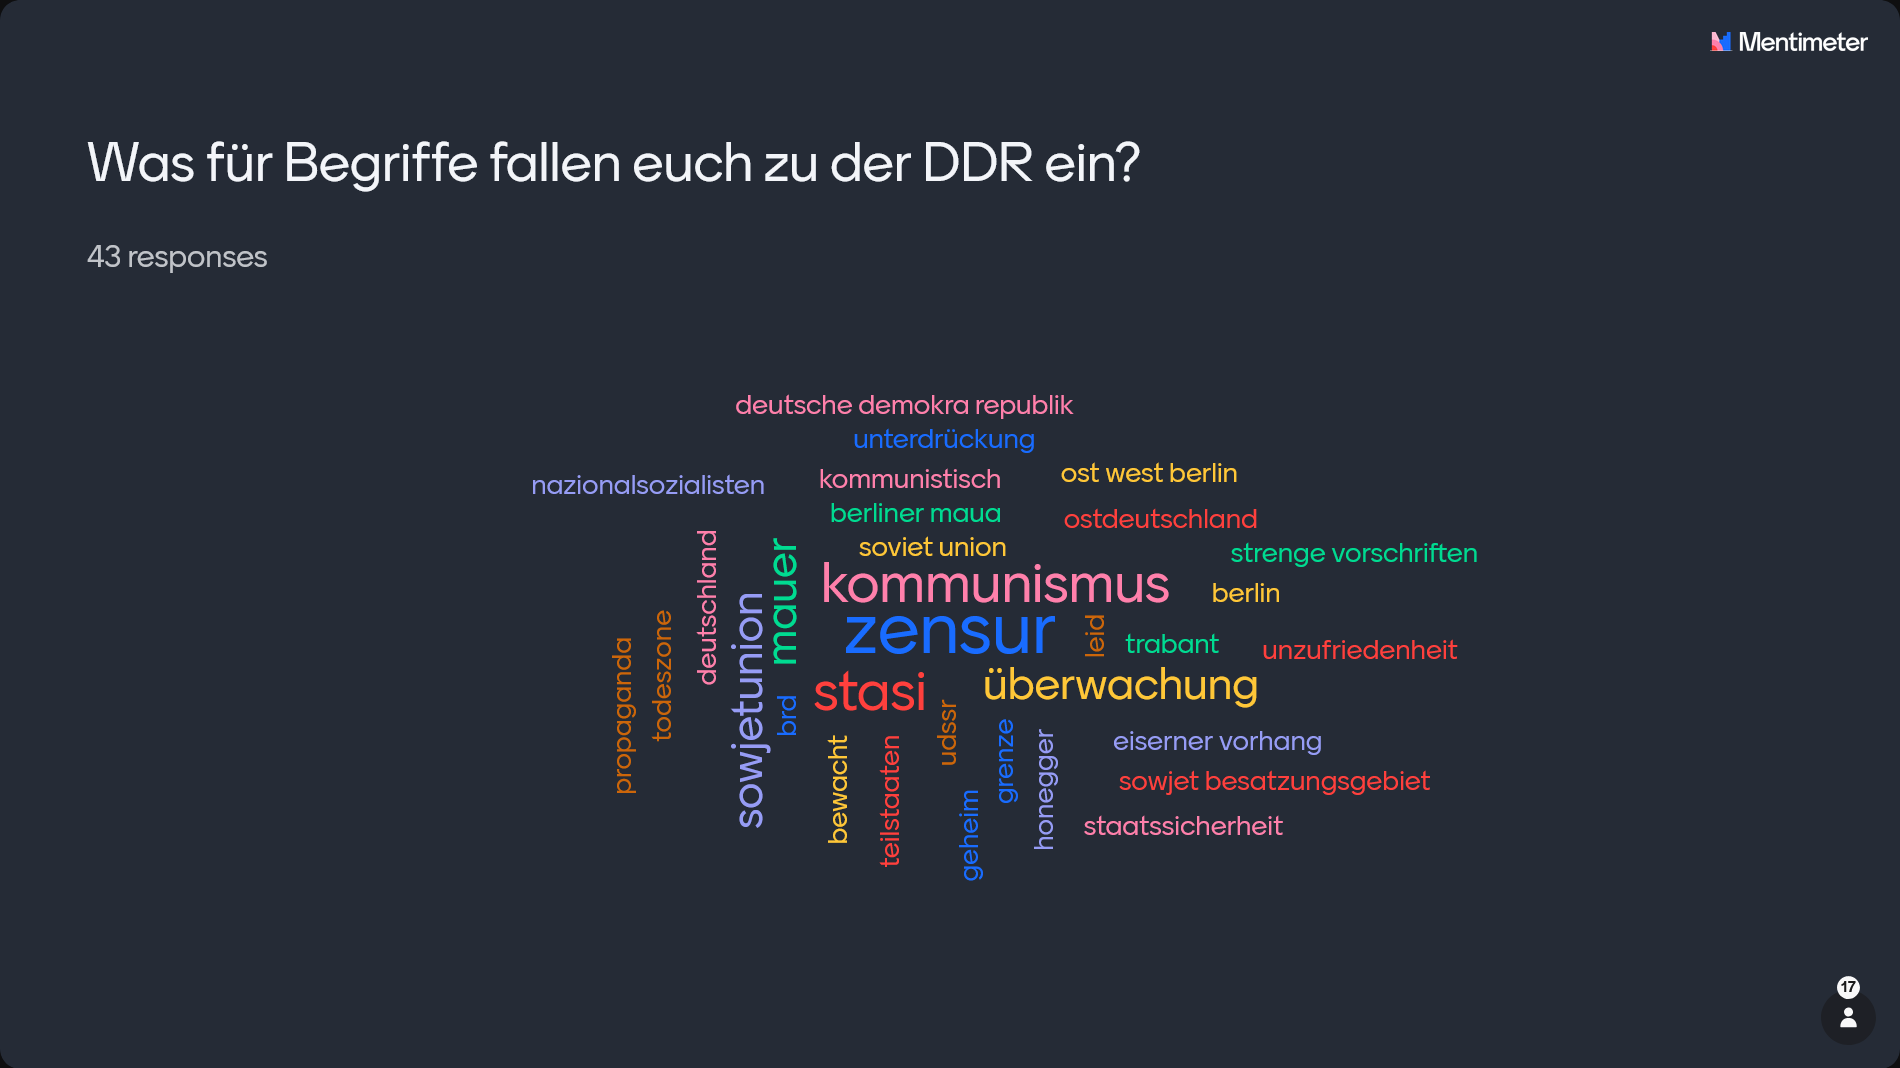
\includegraphics[width=0.5\linewidth]{resources/images/Was_ist_DDR.png}
    \caption{Klassendiskussion DDR}
    \label{fig:Mentimeter}
\end{figure}
Die DDR enstand durch die Niederlage Deutschlands. Es entstand durch die Übernahme durch die Sovjet Union mit der Ost-Mark (unterschiedlich zur BRD) eingeführt. Die DDR verstand sich als sozialistischer Staat auf Basis des Markzismus. Es wurde ähnlich wie die Soviet Union gehandhabt. \\
Die DDR wurde von einer einzelnen Partei - der SED (Sozialistsche Einheitspartei Deutschlands) - regiert. Es ging der Bevölkerung wirtschaftlich und somit allgemein nicht gut und wie wurden diktatorisch regiert. \\
1951 kam es zu einem Aufstand, welcher vom Militär angwewehrt und 1961 kam es dann zum Mauerbau. Die Grenzen wurden nun geschlossen und gegen Aufstand wurde die Stasi (Sttassicherheit) erschaffen. Telefone wurden abgehört und alles wurde untersucht. Man konnte niemandem mehr trauen. Es wurden IM (Inoffizielle Mitarbeiter) eingeführt, welche Freundschaften und Familien ausspionierten. Dadurch wurde der Bevölkerung Angst gemacht.
\subsection{Leben in der DDR}
\textbf{Aufbau (1946 - 1961)}
\begin{itemize}[parsep=0pt]
    \item Rückkehr von Schritstellerin im Exil
    \item Neuaufbau der Gesellschaft
    \item Entgegen des Nationalsozialismus folgte der Sozialismus (Kommunismus) - Es wurde eine Umerziehung durchgeführt
    \item Es wurde die Literatur des Aufbaus geschrieben
\end{itemize}
\textbf{Ankunft (1961 - 1971)}
\begin{itemize}[parsep=0pt]
    \item Es wurde über den Mauerbau geschrieben
    \item Kritik an der DDR und deren Unterdrückung wurde niedergeschrieben
    \item Man versuchte in der Literatur dennoch sich mit der DDR zu versöhnen
    \item Bei dem Bitterferlder Weg trafen sich Schriftsteller, um sich mehr mit der Natur auseinander zu setzen
\end{itemize}
\textbf{Liberaliserung (1971 - 1796)}
\begin{itemize}
    \item Es wurde Kritik erlaubt, solange sie positiv war
\end{itemize}
\textbf{Unterdrückung/Wendung}
\begin{itemize}[parsep=0pt]
    \item Wolf Biermann wurde ausgebürgert
    \item Viele künstler distanzierten sich von der SED, da die Vorgaben strenger wurden. Sie veruchten ihre Message nicht direkt, sondern indirekt einbringen
    \item Gegen ende normalisierte sich die DDR Literatur und ähnelte der BRD Liteatur
\end{itemize}
\section{Literatur (1945-1990)}
\subsection{Aufbauliteratur und Ankunfsliteratur}
\begin{itemize}[parsep=0pt]
    \item \textbf{Es wurde ein Sozialitischer Realismus durchgeführt}
    \item Die Sprache sollte keine sozialen Unterschiede ansprechen und für alle sein
    \item Sie sollten eine klare Erzählstruktur und einfache Sprache haben
    \item Es sollte ein wahrheitsgetreuer Erzählstyl geben, welcher nicht estetisiert ist
    \item sozialistische Protagonisten wurden als Vorbilder der Liteatur genommen
    \item \textbf{Themen:} Individuum gegen Gesellscahft, Kapitalismus als Feind
\end{itemize}
\textbf{Ziel:} sozialistische Erziehung und "Wahrhaftigkeit" der DDR darstellen
\subsection{DDR Kritik}
\begin{itemize}[parsep=0pt]
    \item \textbf{Es war eine Nonkonforme Liteatur}
    \item Als Sprache wurde Jugendsprache verwendet
    \item Kritik wurde verschlüsselt ausgeübt
    \item Es wurde eine untypische Erzählstruktur angewand
\end{itemize}

\section{Die neuen Leiden des jungen W.}
\subsection{Inhalt}

\begin{figure}[h]
    \centering
    \includegraphics[width=0.5\linewidth]{resources/images/Inhaltsangabe_Buch.jpg}
    \caption{Ablauf Inhalt Buch}
    \label{fig:Powerpoint}
\end{figure}

\begin{itemize}[parsep=0pt]
    \item Edgar ist zum aktuellen Zeitpunkt verstorben
    \item Edgars Vater hat die die Familie verlassen und versucht die letzen Monate seines Lebens nachzuvollziehen
    \item Edgar erzählt aus dem "Jehenseits" die Geschehnisse vor seinem Tod.
    \item Der Vater trifft "Charlotte", welche nicht so heisst, welche Edgar kannte, jedoch laut ihrer Aussage nichts romantisches miteinander hatten.
    \item Edgar baute eine Farbspritze, welche in die Luft ging.
    \item Gestorben ist Edgar an einem Stromschlag, welcher von der Farbspritze aus kam, an welcher er selbst bastelte
\end{itemize}

\newpage
\subsection{Auftrag}
\subsubsection{Formanalyse}
\begin{itemize}[parsep=0pt]
    \item Texte von Edgars Vater in der direkten in der Rede
    \item Texte von Edgar in der Erzählinstanz als informativer Text
    \item Tonbänder sind von einer externen Instanz (in diesem Fall Goethe)
    \item Slangwörter: "Changen sind Mau", "Kumpel", "Olle", "ging flöten", "geschmissen"
    \item Euphenismen: Über den Jordan gehen.
    \item \textbf{Vergleich}: Bei den Tonbändern wurde nur wenig auf die Gross-/Kleinschreibung geachtet. Edgar seine Texte sind sehr umfangssprachlich vormuliert und die von Goethe informativ und sachlich. Es werden bei Goethe keine vollständigen Sätze vormuliert.
\end{itemize}
\subsubsection{Inhaltsanalyse}
\begin{itemize}[parsep=0pt]
    \item In beiden Geschichten ist "Charlotte" verlobt / verliebt.
    \item Der Tod mit den Farbspritzen stellt er selbst als Versehen dar.
    \item Er will der Realität entkommen.
    \item Bei beiden ist es eine Kritik an der Zeit, in welcher sie leben.
    \item Eine Jeans ist nur ein Symbol und es spielt an das Gesellschaftsideal eines Körpers an.
    \item Kritik am Kommunismus wurde im letzen Teil des Textes geäussert und man muss nur mutig sein, wenn man dagegen ist und Menschen wollen mutig sein.
\end{itemize}

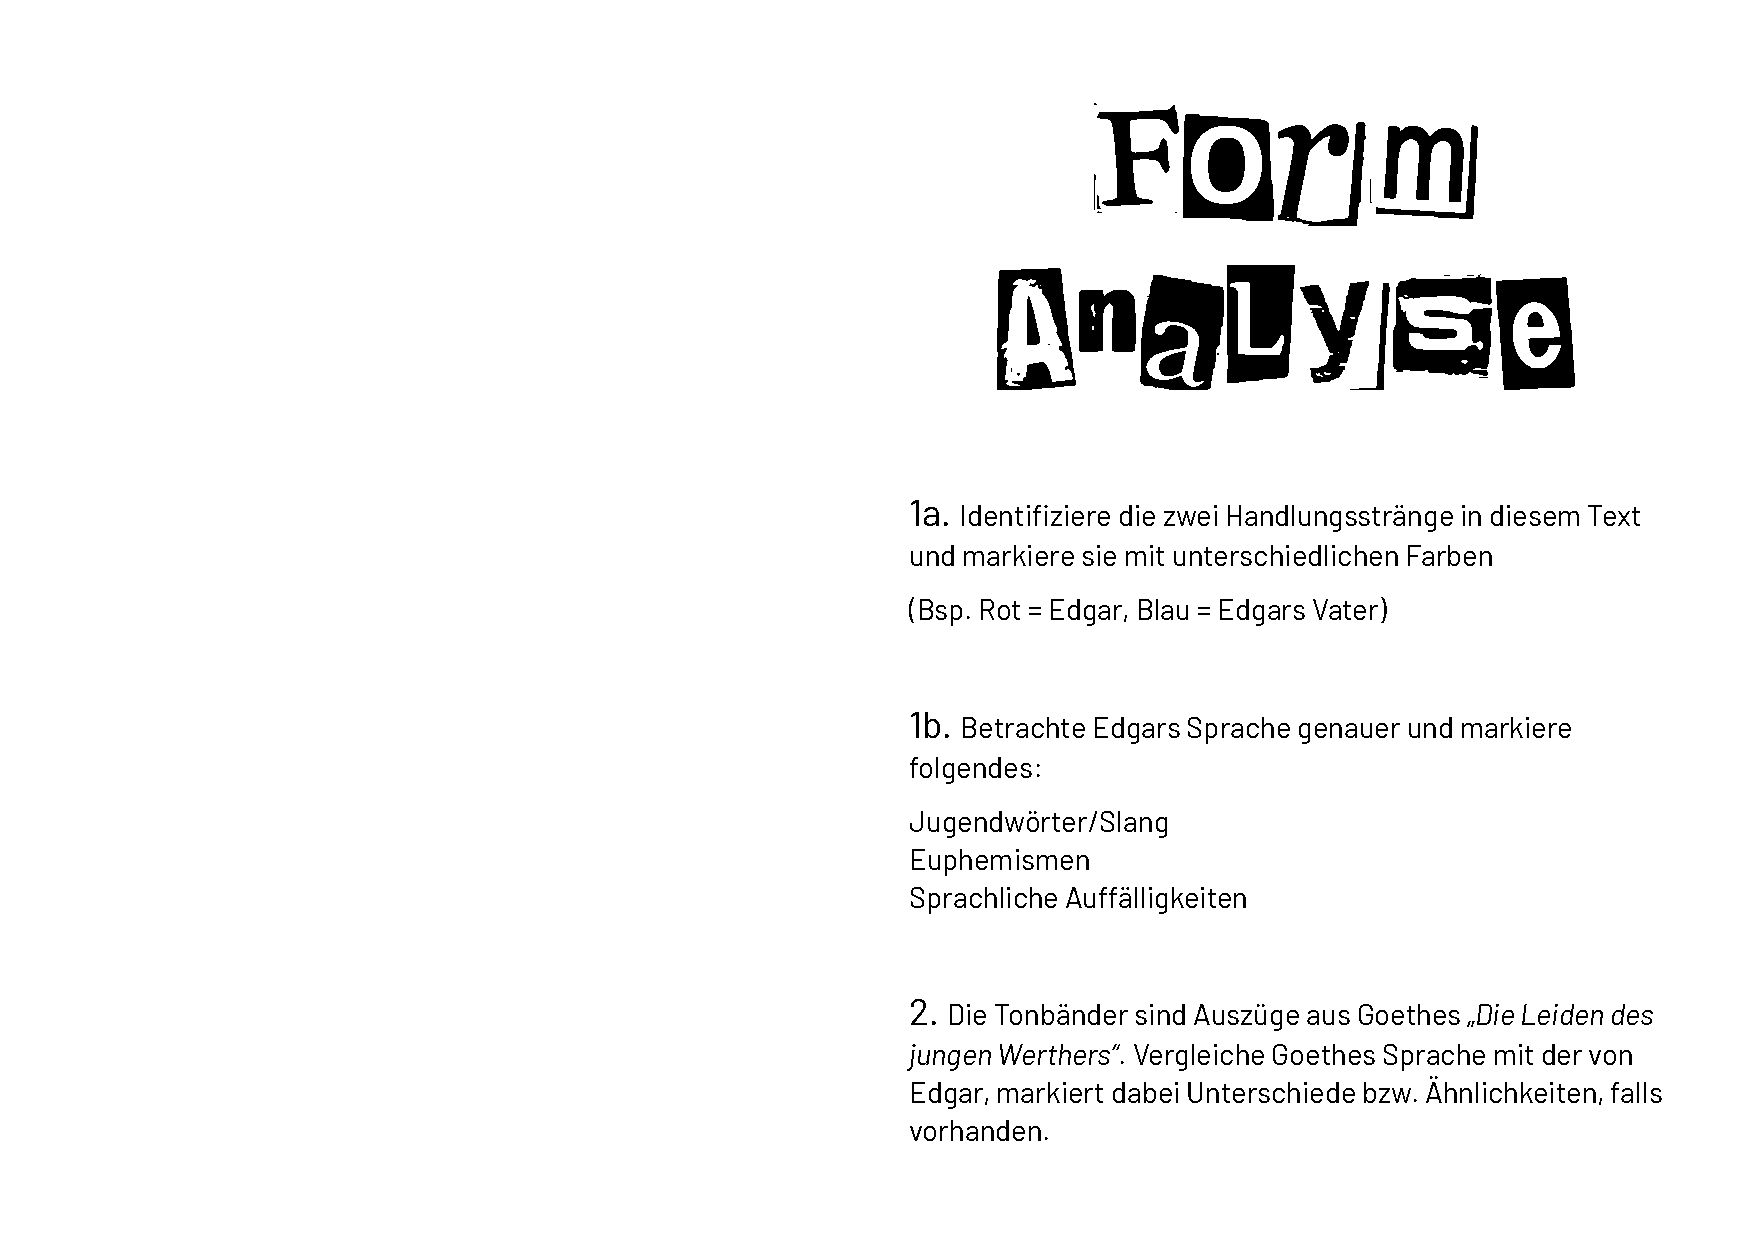
\includepdf[nup=1x2, scale=0.8, pages=-]{resources/pdfs/formanalyse_DDR-1.pdf}
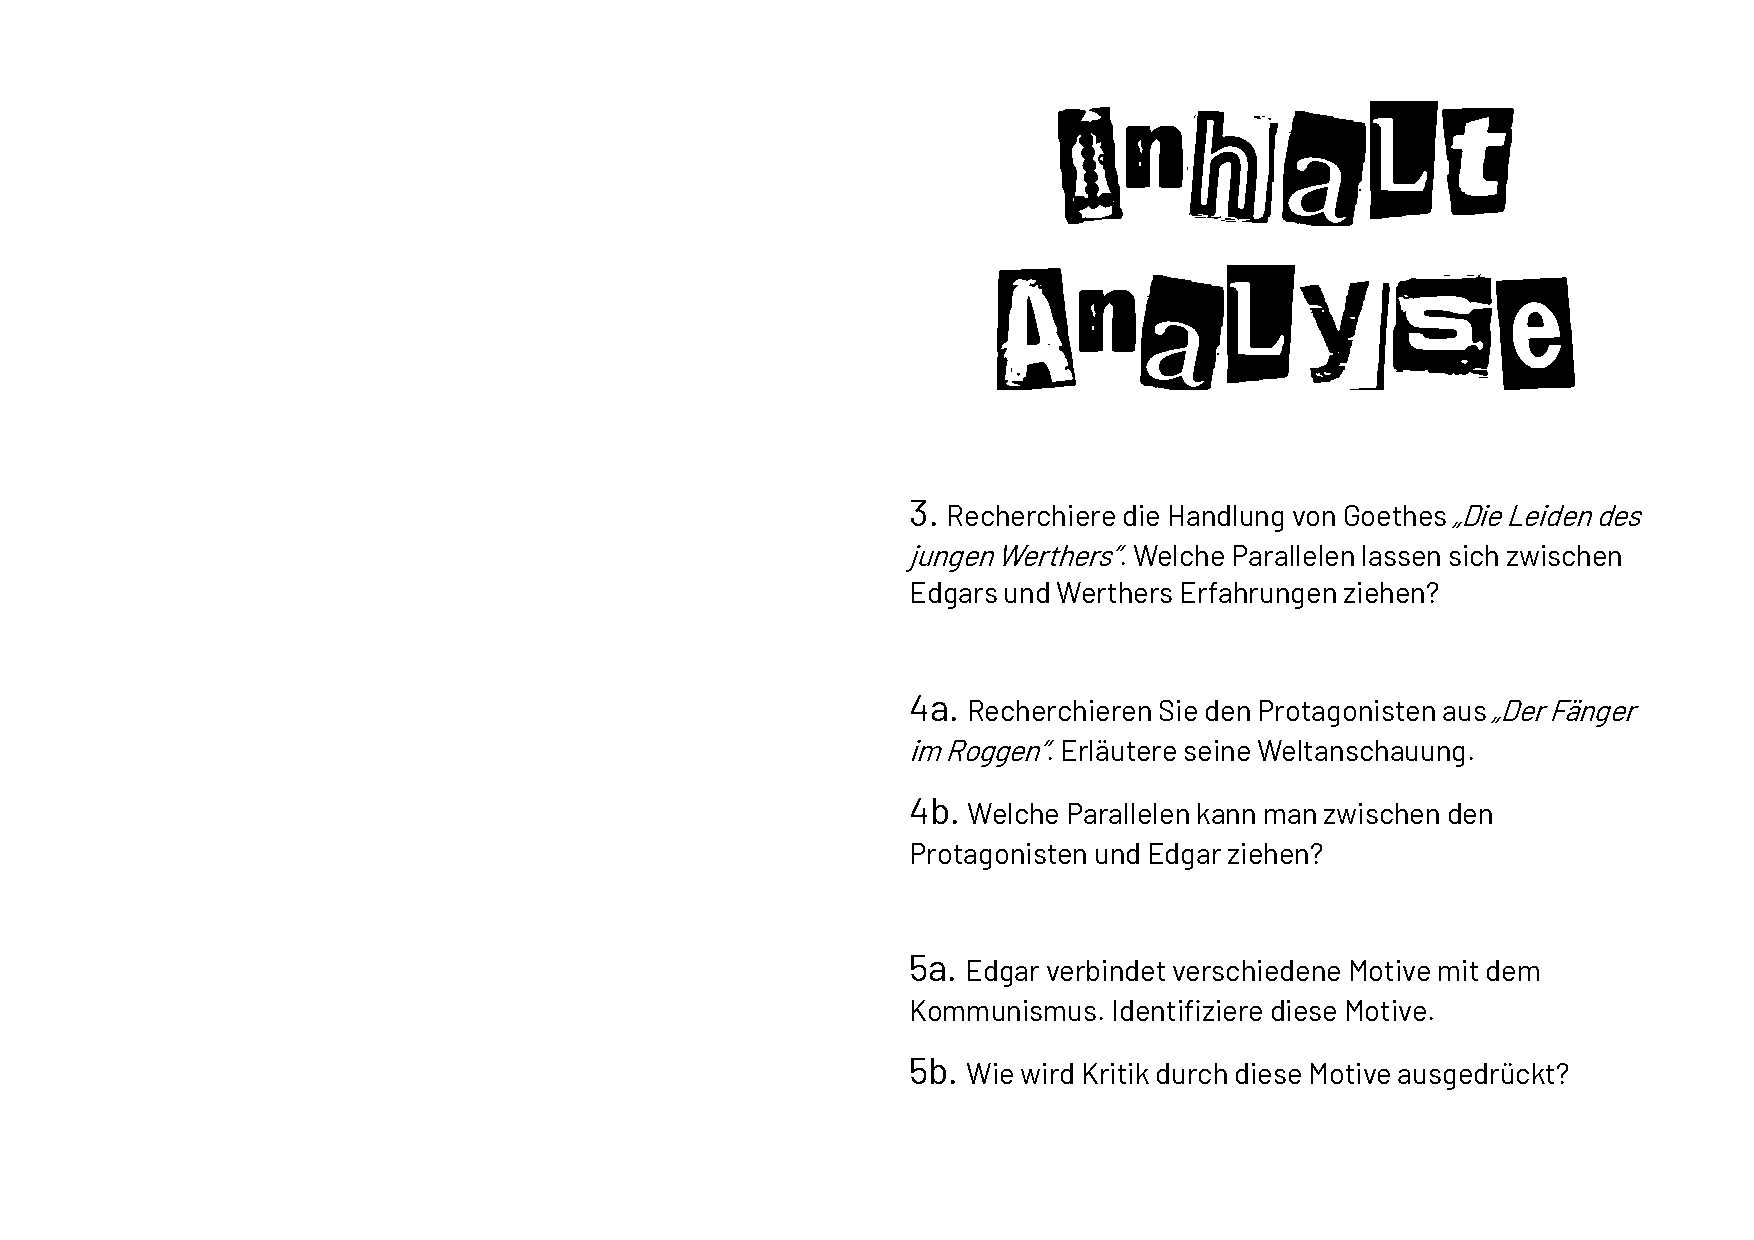
\includepdf[nup=1x2, scale=0.8, pages=-]{resources/pdfs/inhaltanalyse_DDR-1.pdf}

\section{Aktualität}
\begin{itemize}[parsep=0pt]
    \item Das Thema DDR wird immer noch thematisiert
    \item Die Gefühle der Generationen der damaligen Zeit existieren immer noch
    \item Es gibt immer noch Unterdrückungen, welche auch heute noch in der Literatur beschäftigt.
    \item Die Unterdrückung wurde auf die feministische Benachteiligung übertragen.
\end{itemize}
\end{document}
